\chapter{Tetis - Modelagem e Controle}

\section{Parâmetros Denavit–Hartenberg}

\begin{figure}[!ht]
\centering
  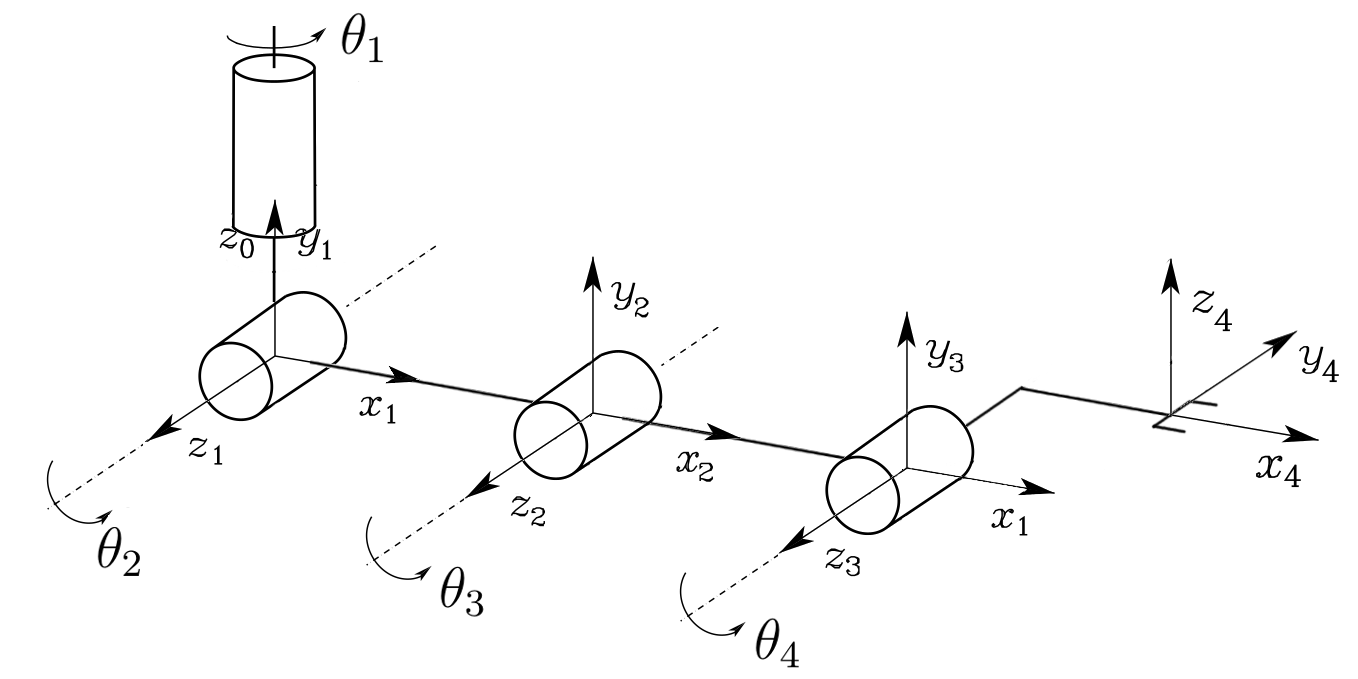
\includegraphics[width=0.9\linewidth]{./img/m2_meio_2.png}
  \caption{Modelagem do Manipulador Tetis e posicionamento dos sistemas de coordenadas}
  \label{fig:modelo_tetis}
\end{figure}%

\begin{table}[!ht]
\centering
\caption{Parâmetros Denavit–Hartenberg para manipulatodor Tetis}
\label{tab:dh_tetis}
\begin{tabular}{rrrrr} \hline
Elo & $a_i$ & $\alpha_i$ & $d_i$  & $\theta_i$ \\ \hline
1   & 0     & $\pi/2$    & 0      & $\theta_1$ \\
2   & $E_3$ & 0          & 0      & $\theta_2$ \\
3   & $E_4$ & 0          & 0      & $\theta_3$ \\
4   & $E_5$ & $-\pi/2$   & $-M_5$ & $\theta_4$ \\ \hline
\end{tabular}
\end{table}

\section{Cinemática Direta}

\begin{equation}
\bm{R}_{i-1,i} = \bm{R}_z(\theta_i)\bm{R}_x(\alpha_i)
\end{equation}
\begin{equation}
\bm{\vec{p}}_{i-1,i} = d_i \bm{\vec{z}}_{i-1} + a_i \bm{\vec{x}}_i
\end{equation}
\begin{gather}
(\bm{\vec{p}}_{i-1,i})_{i-1} = d_i (\bm{\vec{z}}_{i-1})_{i-1} + a_i (\bm{\vec{x}}_i)_{i-1} \\
(\bm{\vec{p}}_{i-1,i})_{i-1} = d_i (\bm{\vec{z}}_{i-1})_{i-1} + a_i \bm{R}_{i-1,i}(\bm{\vec{x}}_i)_{i} 
\end{gather}

%\begin{align*}
%\bm{R}_{01} =
%\m{c_1 & 0 & s_1   \\
%   s_1 & 0 & -c_1  \\
%   0   & 1 &    0  \\} 
%& & \vec{\bm{p}}_{01} = 0
%\end{align*}
%\begin{align*}
%R_{12} = 
%\m{c_2 & -s_2 &  0  \\
%   s_2 &  c_2 &  0  \\
%   0   &    0 &  1  \\} 
%\end{align*}
%\begin{align*}
%R_{23} = 
%\m{c_3 & -s_3 &  0  \\
%   s_3 &  c_3 &  0  \\
%   0   &    0 &  1  \\} 
%\end{align*}
%\begin{align*}
%R_{34} = 
%\m{c_4 &  0 & -s_4  \\
%   s_4 &  0 &  c_4  \\
%   0   & -1 &    0  \\} 
%\end{align*}


%\begin{equation}
%\bm{R}_{04} = 
%\m{
%	c_1 c_{234} & -s_1 & -c_1 s_{234} \\
%	s_1 c_{234} & -c_1 & -s_1 s_{234} \\
%		s_{234} &    0 & 	  c_{234}
%}
%\end{equation}


\[ \bm{T}_{01} = 
\m{c_1 & 0 & s_1 &  0 \\
   s_1 & 0 & -c_1 & 0 \\
   0   & 1 &    0 & 0 \\
   0   & 0 &    0 & 1}\]

\[ \bm{T}_{12} = 
\m{c_2 & -s_2 &  0 & E_3 c_2 \\
   s_2 &  c_2 &  0 & E_3 s_2  \\
   0   &    0 &  1 & 	   0  \\
   0   &    0 &  0 &       1} \]

\[ \bm{T}_{23} = 
\m{c_3 & -s_3 &  0 & E_4 c_3 \\
   s_3 &  c_3 &  0 & E_4 s_3  \\
   0   &    0 &  1 & 	   0  \\
   0   &    0 &  0 &       1} \]

\[ \bm{T}_{34} = 
\m{c_4 &    0 &  -s_4 & E_5 c_4 \\
   s_4 &    0 &   c_4 & E_5 s_4 \\
   0   &   -1 &     0 & 	-M_5 \\
   0   &    0 &     0 &       1} \]

\begin{equation} \label{eq:cine_direta}
 \bm{T}_{04} = \bm{T}_{01} \bm{T}_{12}  \bm{T}_{23} \bm{T}_{34} = 
\m{
   c_1 c_{234} & -s_1 & -c_1 s_{234} & -M_5 s_1 + E_4 c_{23}c_1 + E_3 c_1 c_2 + E_5 c_{234} c_1 \\
   s_1 c_{234} & -c_1 & -s_1 s_{234} &   M_5 c_1+E_4 c_{23} s_1 + E_3 c_2 s_1 + E_5 c_{234} s_1 \\
   s_{234}     &    0 &      c_{234} &					     E_4 s_{23} + E_3 s_2 + E_5 s_{234} \\
   0   &    0 &     0 &      												   1
} 
\end{equation}

\section{Espaço das Juntas e Operacional}
Antes de tratar de estratégias de controle é necessário definir o espaço operacional e o espaço das juntas,  sob os quais serão aplicadas as leis de controle. 
Como trata-se de um manipulador 4-DOF de temos que o vetor do espaço operacional tem dimensão $(4 \times 1)$ dado por 
\begin{equation}
\bm{x_e} = \m{\bm{p}_e \\ \phi_e}
\end{equation}
onde o vetor $\bm{p}_e$ descreve a posição cartesiana representada no referencial da base:
\begin{equation}
\bm{p}_e = \m{x \\ y \\ z}
\end{equation}
e $\phi_e$ é o grau de liberdade de orientação \textit{pitch} no referencial do efetuador (??), dado por
\begin{equation} \label{eq:orientacao}
\phi_e = -(\theta_2 + \theta_3 + \theta_4)
\end{equation}

O espaço das juntas é definido por 
\begin{equation} \label{joint_space}
\bm{q} = \m{q_1 \\ q_2 \\ q_3 \\ q_4} = \m{\theta_1 \\ \theta_2 \\ \theta_3 \\ \theta_4  }
\end{equation} 
pois todas as juntas são de revolução.

\section{Cinemática Diferencial}

\subsection{Jacobiano Analítico}
A partir da cinemática direta em \eqref{eq:cine_direta} e da equação \ref{eq:jacob_pos} podemos obter o Jacobiano de Posição para o manipulador diferenciando a equação em relação as variáveis de junta.

\begin{equation}
\bm{p}_e = \m{x \\ y \\ z} =
\m{
   -M_5 s_1 + E_4 c_{23}c_1 + E_3 c_1 c_2 + E_5 c_{234} c_1 \\
     M_5 c_1+E_4 c_{23} s_1 + E_3 c_2 s_1 + E_5 c_{234} s_1 \\
   						 E_4 s_{23} + E_3 s_2 + E_5 s_{234} \\
}
\end{equation}

\begin{equation}
(\bm{J}_P)_0 = 
\m{
	\ddfrac{\partial x}{\partial q_1} & \ddfrac{\partial x}{\partial q_2} & \ddfrac{\partial x}{\partial q_3} & \ddfrac{\partial x}{\partial q_4}  \\
	\ddfrac{\partial y}{\partial q_1} & \ddfrac{\partial y}{\partial q_2} & \ddfrac{\partial y}{\partial q_3} & \ddfrac{\partial x}{\partial q_4}  \\
	\ddfrac{\partial z}{\partial q_1} & \ddfrac{\partial z}{\partial q_2} & \ddfrac{\partial z}{\partial q_3} & \ddfrac{\partial z}{\partial q_4}  \\
}
\end{equation}
onde
\begin{align*}
&\frac{\partial x}{\partial q_1} =& - M_5c_1 - E_4c_{23}s_1 - E_3c_2s_1 - E_5c_{234}s_1  \\
&\frac{\partial x}{\partial q_2} =& -c_1(E_4s_{23}+E_3s_2+E_5s_{234}) \\
&\frac{\partial x}{\partial q_3} =& -c_1(E_4s_{23}+E_5s_{234}) \\
&\frac{\partial x}{\partial q_4} =& -E_5s_{234}c_1 \\
&\frac{\partial y}{\partial q_1} =& -M_5s_1+E_4c_{23}c_1+E_3c_1c_2+E_5c_{234}c_1 \\
&\frac{\partial y}{\partial q_2} =& -s_1(E_4s_{23}+E_3s_2+E_5s_{234}) \\
&\frac{\partial y}{\partial q_3} =& -s_1(E_4s_{23}+E_5s_{234}) \\
&\frac{\partial y}{\partial q_4} =& -E_5s_{234}s_1 \\ 
&\frac{\partial z}{\partial q_1} =& 0 \\ 
&\frac{\partial z}{\partial q_2} =& E_4c_{23}+E_3c_2+E_5c_{234} \\
&\frac{\partial z}{\partial q_3} =& E_4c_{23}+E_5c_{234}\\
&\frac{\partial z}{\partial q_4} =& E_{5}c_{234} 
\end{align*}

A partir de \ref{eq:jacob_or} e de \ref{eq:orientacao} podemos calular o Jacobiano de Orientação
\begin{equation}
\bm{J}_{\phi}(\bm{q}) = \frac{\partial \phi_e}{\partial \bm{q}} = \m{0 & -1 & -1 & -1}
\end{equation}
 
Em alguns modos como controle por servo visão e no controle manual com joystick é interessante fazer o controle no referêncial do efetuador, portanto precisamos representar o Jacobiano de posição no referencial do efetuador como $(\bm{J}_P)_N = \bm{R}_{04}^T (\bm{J}_P)_0$.  

\begin{equation}
(\bm{J}_P)_N =  
\m{
    -M_5c_{234} & E_3s_{34}+E_4s_4 & E_4s_4 & 0 \\
    E_4c_{23}+E_3c_2+E_5c_{234} & 0 & 0 & 0 \\
    M_5s_{23} &  E_5+E_3c_{34}+E_4c_4 & E_5+E_4c_4 & E_5 
}
\end{equation}
\section{Singularidades}


\section{Modos de Controle}
\subsection{Velocidade no Espaço Operacional}
Neste modo é uma malha aberta, onde enviamos comandos de velocidade 
\subsubsection{Base}
\subsubsection{Efetuador}
\subsection{Posição no Espaço das Juntas}
\subsection{Posição no Espaço Operacional}
Para este modo considera-se o problema de controle de posição no espaço operacional conforme definido em \ref{eq:op_space}. 

\subsection{Rastreamento de Trajetória}

\subsection{Servo Visão}
\subsection{Força}
\subsubsection{Float}
\subsubsection{Approach}
Considera-se o problema de controle de força na direção de approach para o manipulador robótico 4-DOF em questão. A realimentação de força é feita com o uso do sensor descrito em \ref{sec:sensor_forca}. O objetivo de controle é rastrear uma entrada na forma de um degrau de força, a ser aplicada em uma placa de poliestireno montada em um suporte fixado na verical como mostra a figura \ref{fig:suporte_forca}.  

É possível modelar o ambiente (força de contato), ou seja, a placa de poliestireno como uma mola linear, através da \textit{Lei de Hook}: \cite{bib:toni}
\begin{equation}
f = -k_s (x - x_s)
\end{equation}
onde $x$ é o ponto de contato com a superfície e $x_s$
\subsubsection{Híbrido}
\subsection{Master-Slave (Omni)}
